%
% LaTeX report template 
%
\documentclass[a4paper,12pt]{article}
\usepackage{graphicx}
\usepackage[english]{babel}
\usepackage{fontspec}
\usepackage{listings}
\usepackage{xcolor}
%
% set python code style
\definecolor{codegreen}{rgb}{0,0.6,0}
\definecolor{codegray}{rgb}{0.5,0.5,0.5}
\definecolor{codepurple}{rgb}{0.58,0,0.82}
\definecolor{backcolour}{rgb}{0.95,0.95,0.92}
\lstdefinestyle{pystyle}{
	backgroundcolor=\color{backcolour},   
	commentstyle=\color{codegreen},
	keywordstyle=\color{magenta},
	numberstyle=\tiny\color{codegray},
	stringstyle=\color{codepurple},
	basicstyle=\ttfamily\footnotesize,
	breakatwhitespace=false,         
	breaklines=true,                 
	captionpos=b,                    
	keepspaces=true,                 
	numbers=left,                    
	numbersep=5pt,                  
	showspaces=false,                
	showstringspaces=false,
	showtabs=false,                  
	tabsize=2
}
\lstset{style=pystyle}
%
%font
\setmainfont{Times New Roman}
%
%figure space
%
\setlength{\abovecaptionskip}{0.cm}
\setlength{\belowcaptionskip}{0.cm}   %???????????
%
%
%start document
\begin{document}
%
   \title{\textbf{DSP assignment1 report}}

   \author{Jingyan Wang, 2533494w \\ Qianqian Wang , 2595993w}
          
   \date{}

   \maketitle
   
   \tableofcontents
 
  \newpage
% after a "%" symbol is treated as comment

\section{Task1}
The record can be found in \lstinline|"./Resources/original.wav"|
\section{Task2}
The time domain is as Figure\ref{fig_recordT}, the frequency domain is as Figure\ref{fig_recordF}
\begin{figure}[h]   
	\centering 
	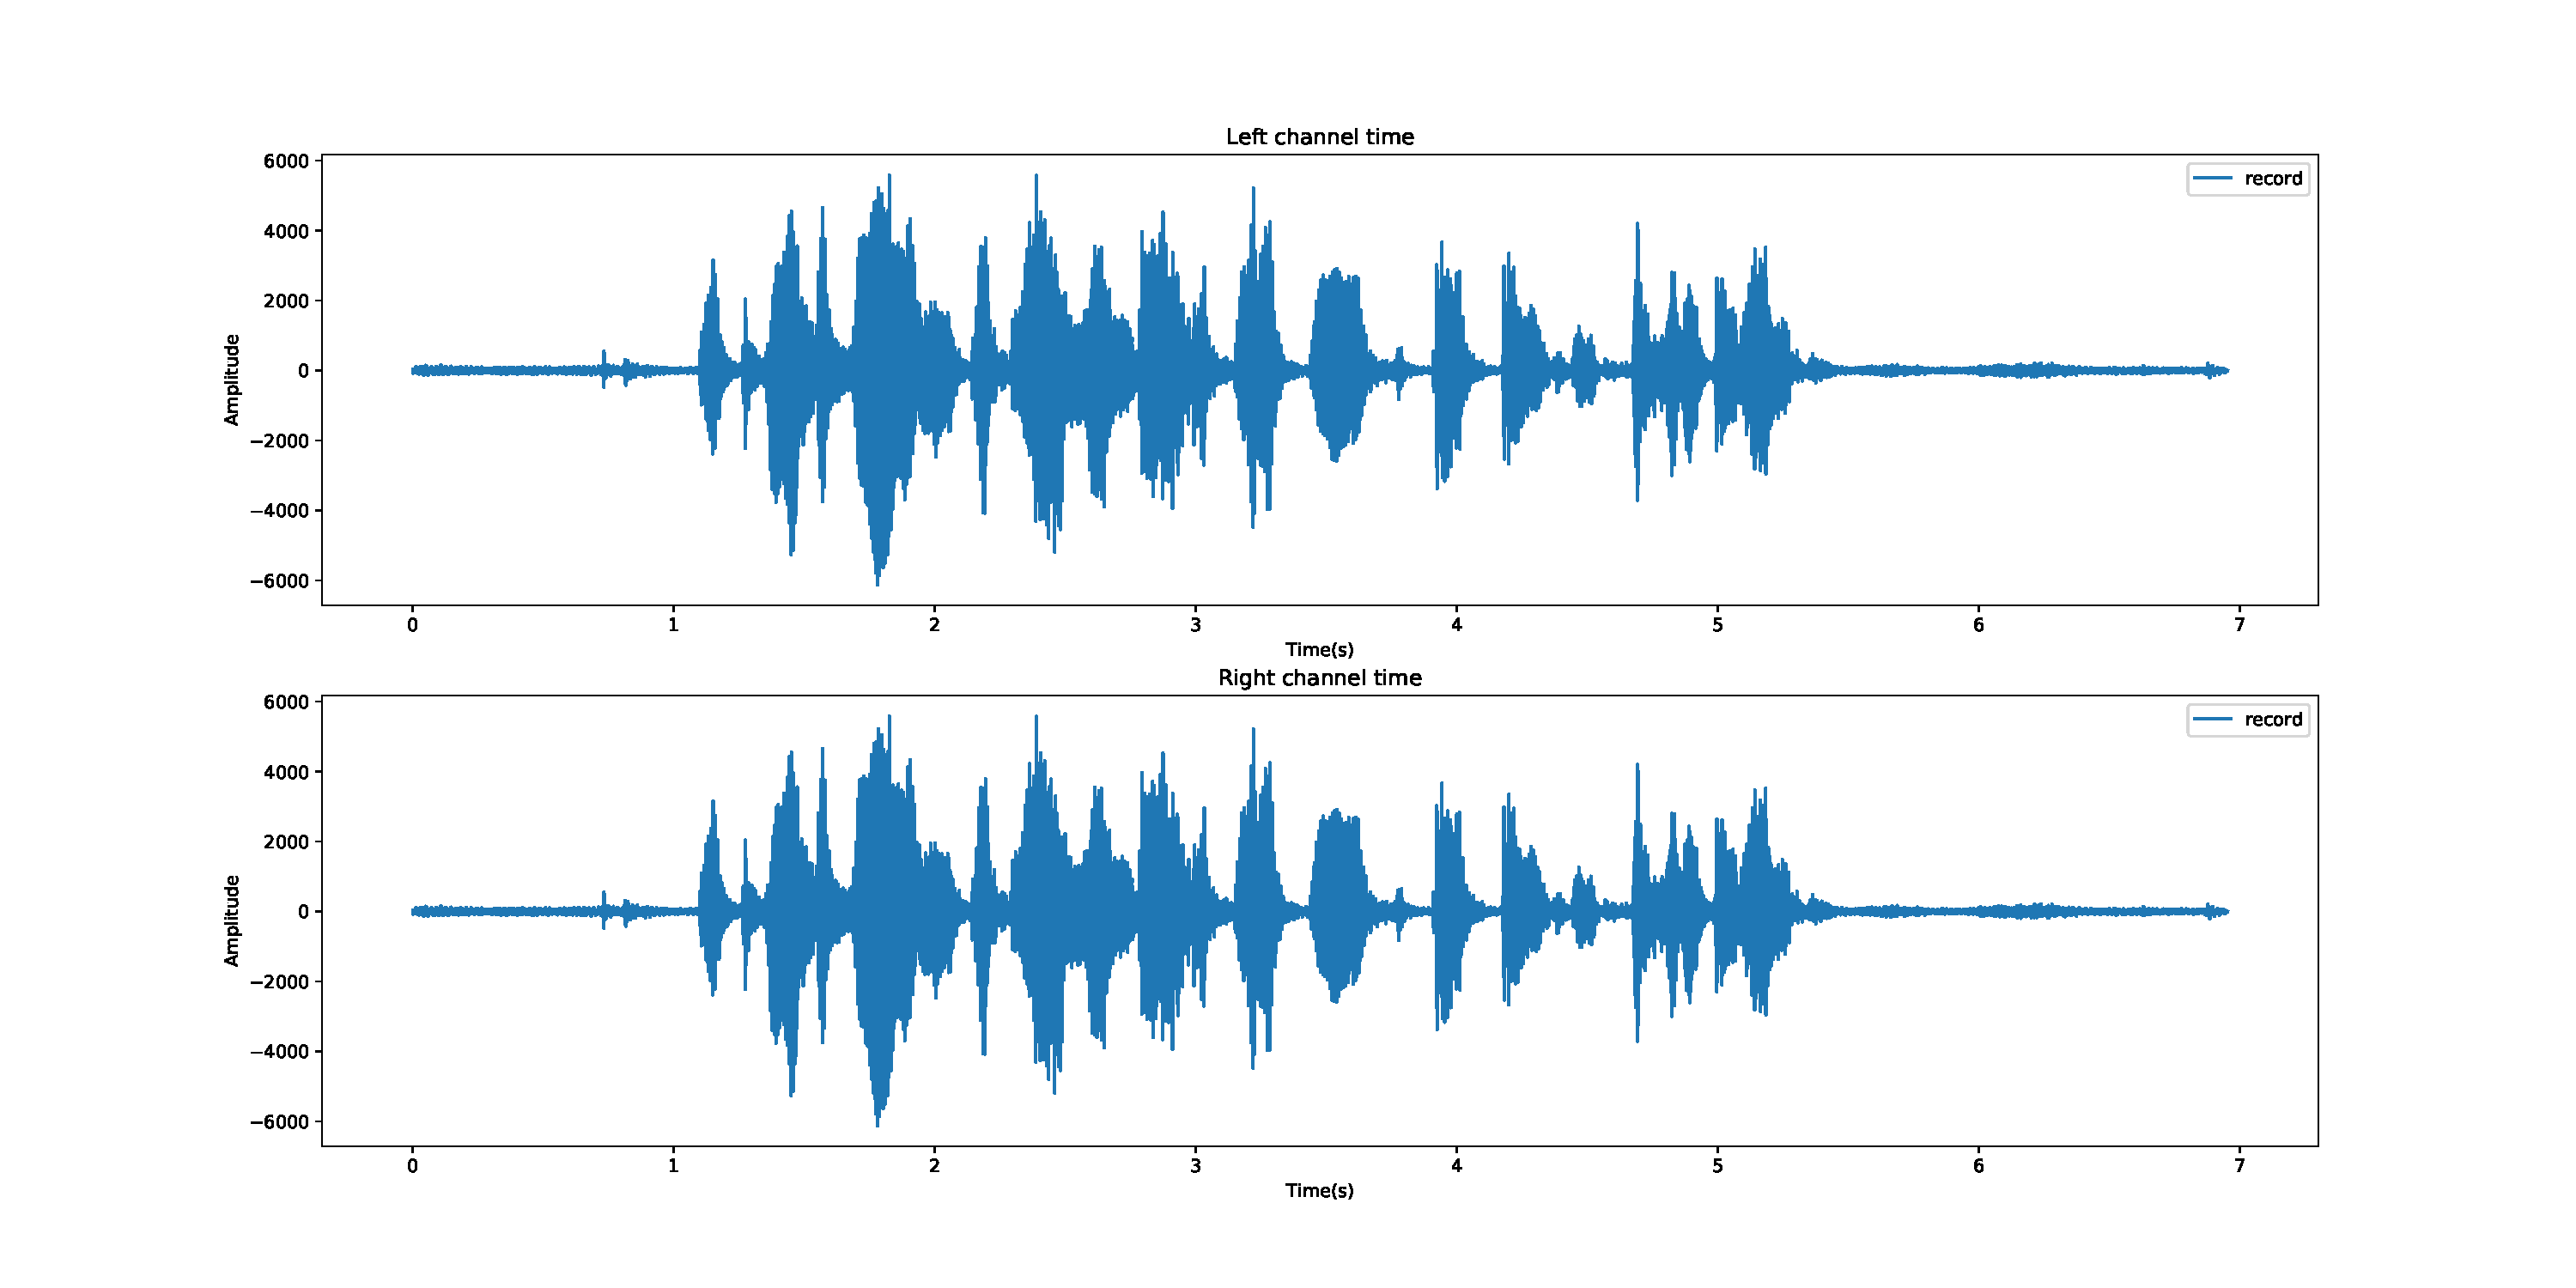
\includegraphics[width=12cm]{../Output/Figures/recordT} 
	\caption{time domain}   
	\label{fig_recordT}
\end{figure}
\begin{figure}[h]   
	\centering 
	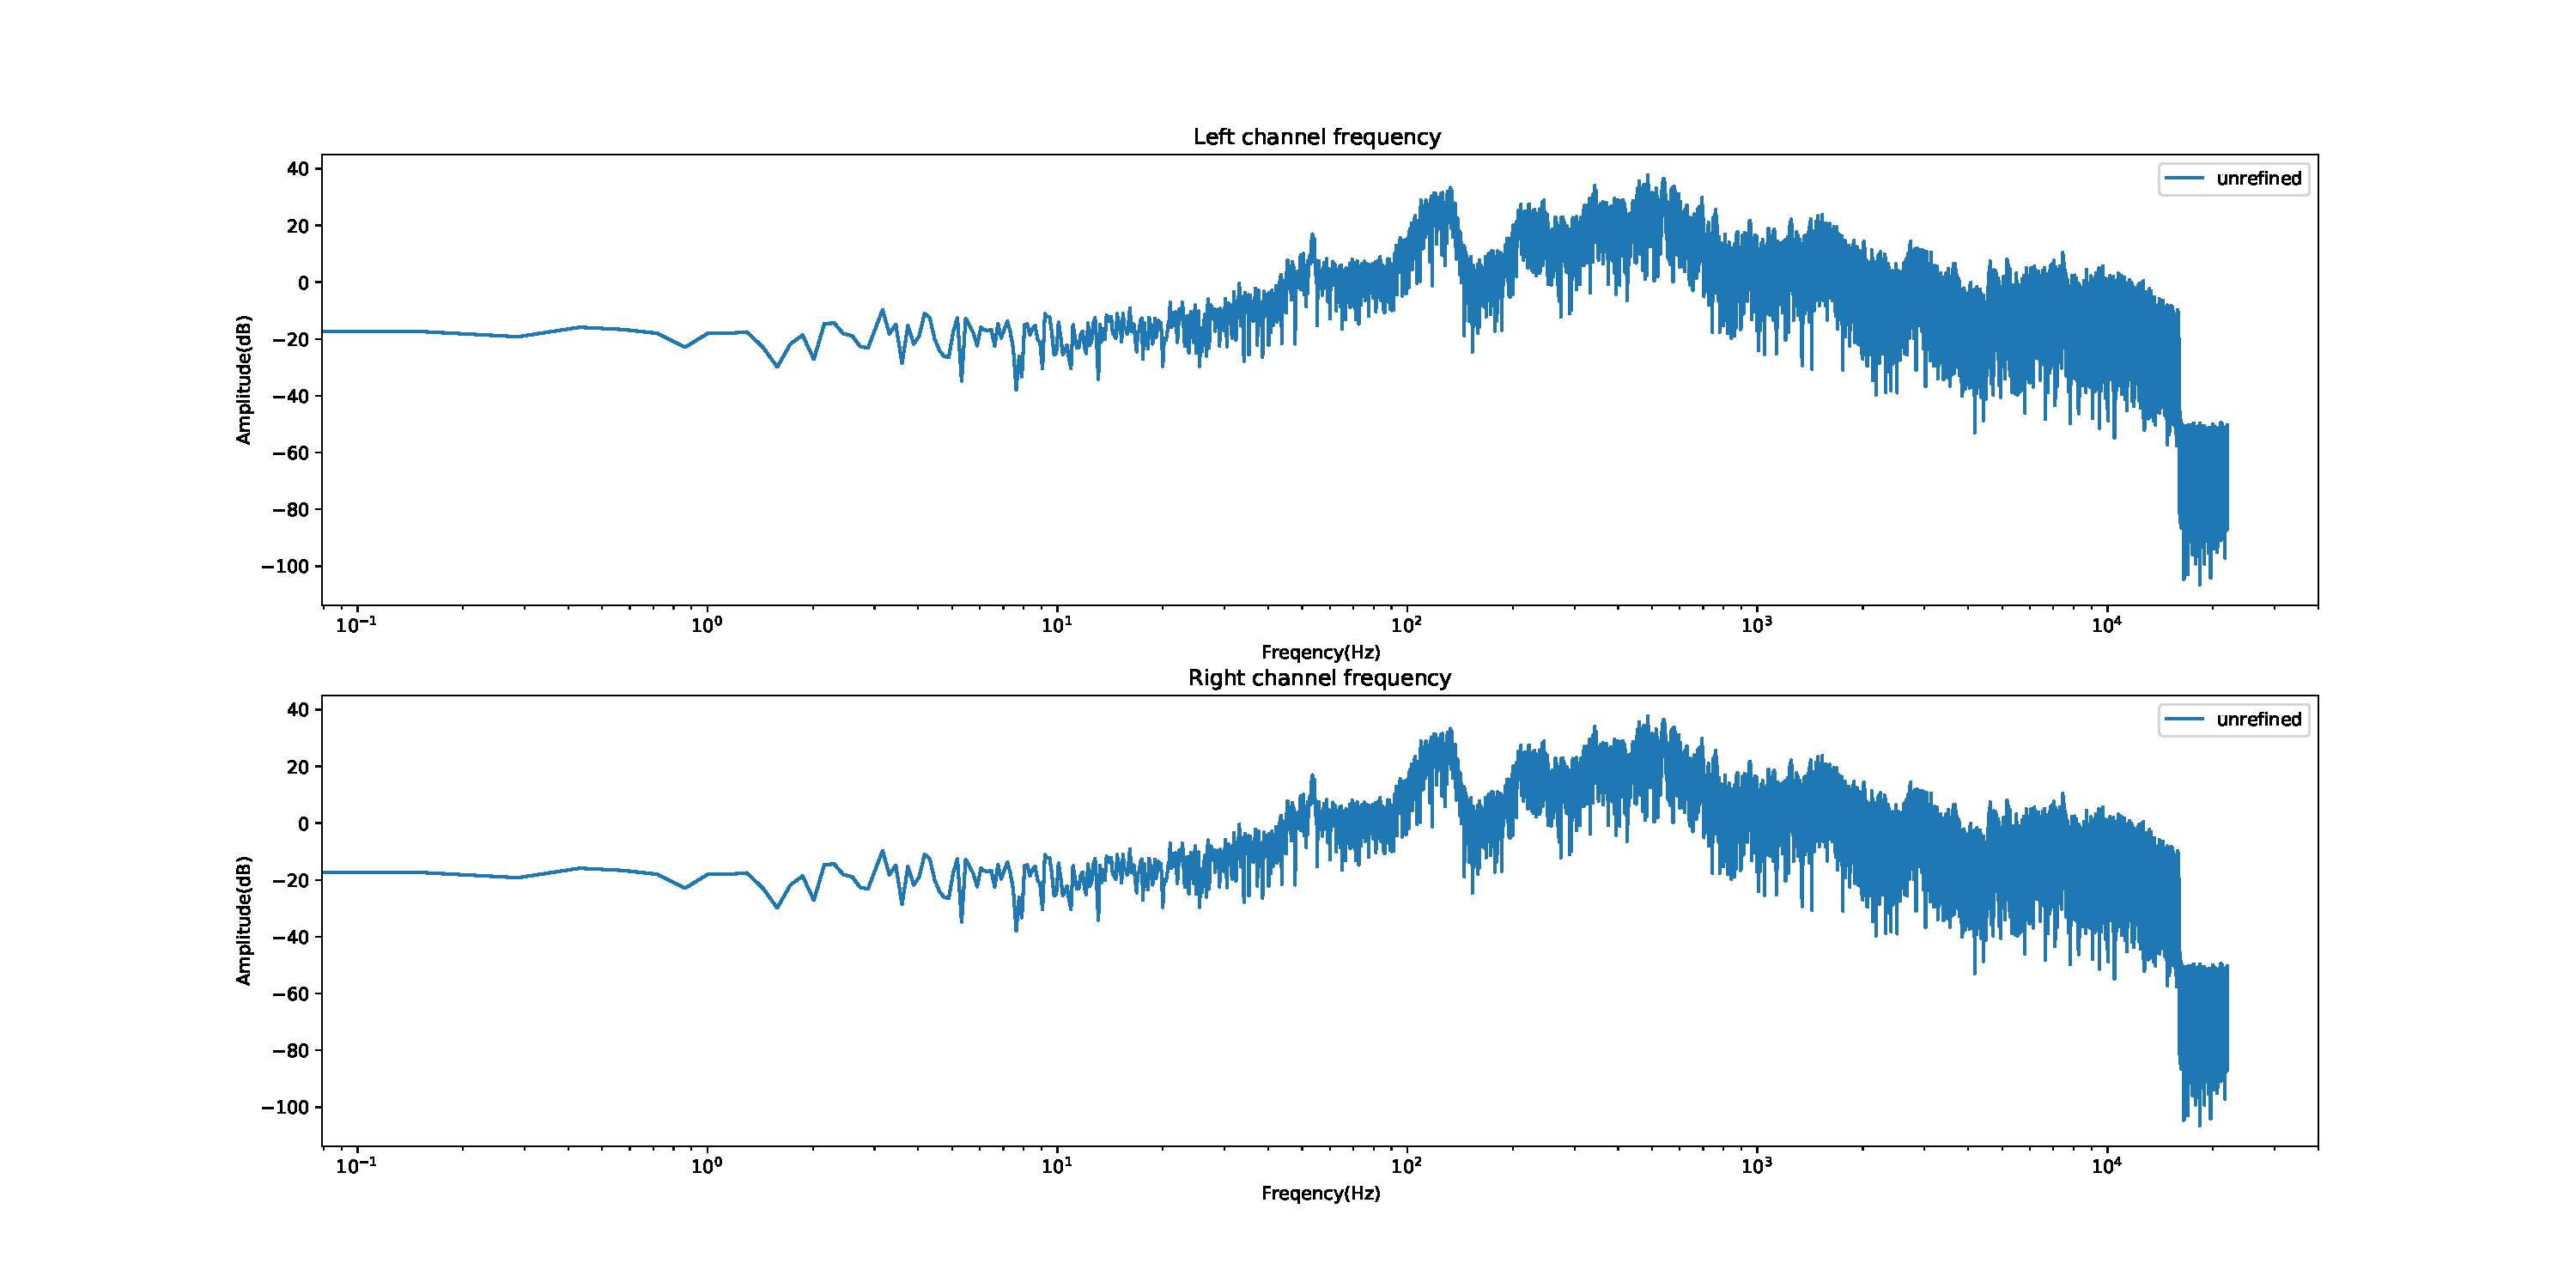
\includegraphics[width=12cm]{../Output/Figures/recordF} 
	\caption{frequency domain}   
	\label{fig_recordF}
\end{figure}
\section{Task3}
As shown by Figure\ref{fig_recordF}, the vowel fundamental frequency is around 127Hz, and the containing the consonants is around  170-4200Hz
\section{Task4}
To amplify the amplitude of the waveform,  we created a window function(Figure\ref{fig_window}) whose amplitude is 5 in 120-900Hz and 6K-10KHz. Then,  multiplied it with the frequency domain of the original signal (amplify the original signal 5 times in both base and higher frequency range):
$$f_{out}=f*f_{window}$$
Finally, we turn it back to a time series by ifft:
\begin{lstlisting}[language=Python]
w = np.ones(N)
modifyWindow(w, 120, 900, rate, 5)
modifyWindow(w, 6000, 10000, rate, 5)

lchannelfRefine = lchannelf*w
rchannelfRefine = rchannelf*w

lchannelRefine = np.fft.ifft(lchannelfRefine)
rchannelRefine = np.fft.ifft(rchannelfRefine)

def modifyWindow(w, startFreqency, endFreqency, sampleRate, value):
	"""modify the window function into rectangular form"""
	beginPoint = int(startFreqency//(sampleRate/N))
	endPoint = int(endFreqency//(sampleRate/N))
	
	w[beginPoint:endPoint] = value
	w[-endPoint:-beginPoint] = value
\end{lstlisting}
we could find the variation in both time domain and frequency domain with Figure\ref{fig_recordTR} and Figure\ref{fig_recordFR}\\
Finally, Ouput the wavefile in \lstinline{"./Output/improved.wav"}:
\begin{lstlisting}[language=Python]
writeWavefile(outputWaveAddress, rate, lchannelRefine.astype(np.int16), rchannelRefine.astype(np.int16))
\end{lstlisting}
\begin{figure}[h]   
	\centering 
	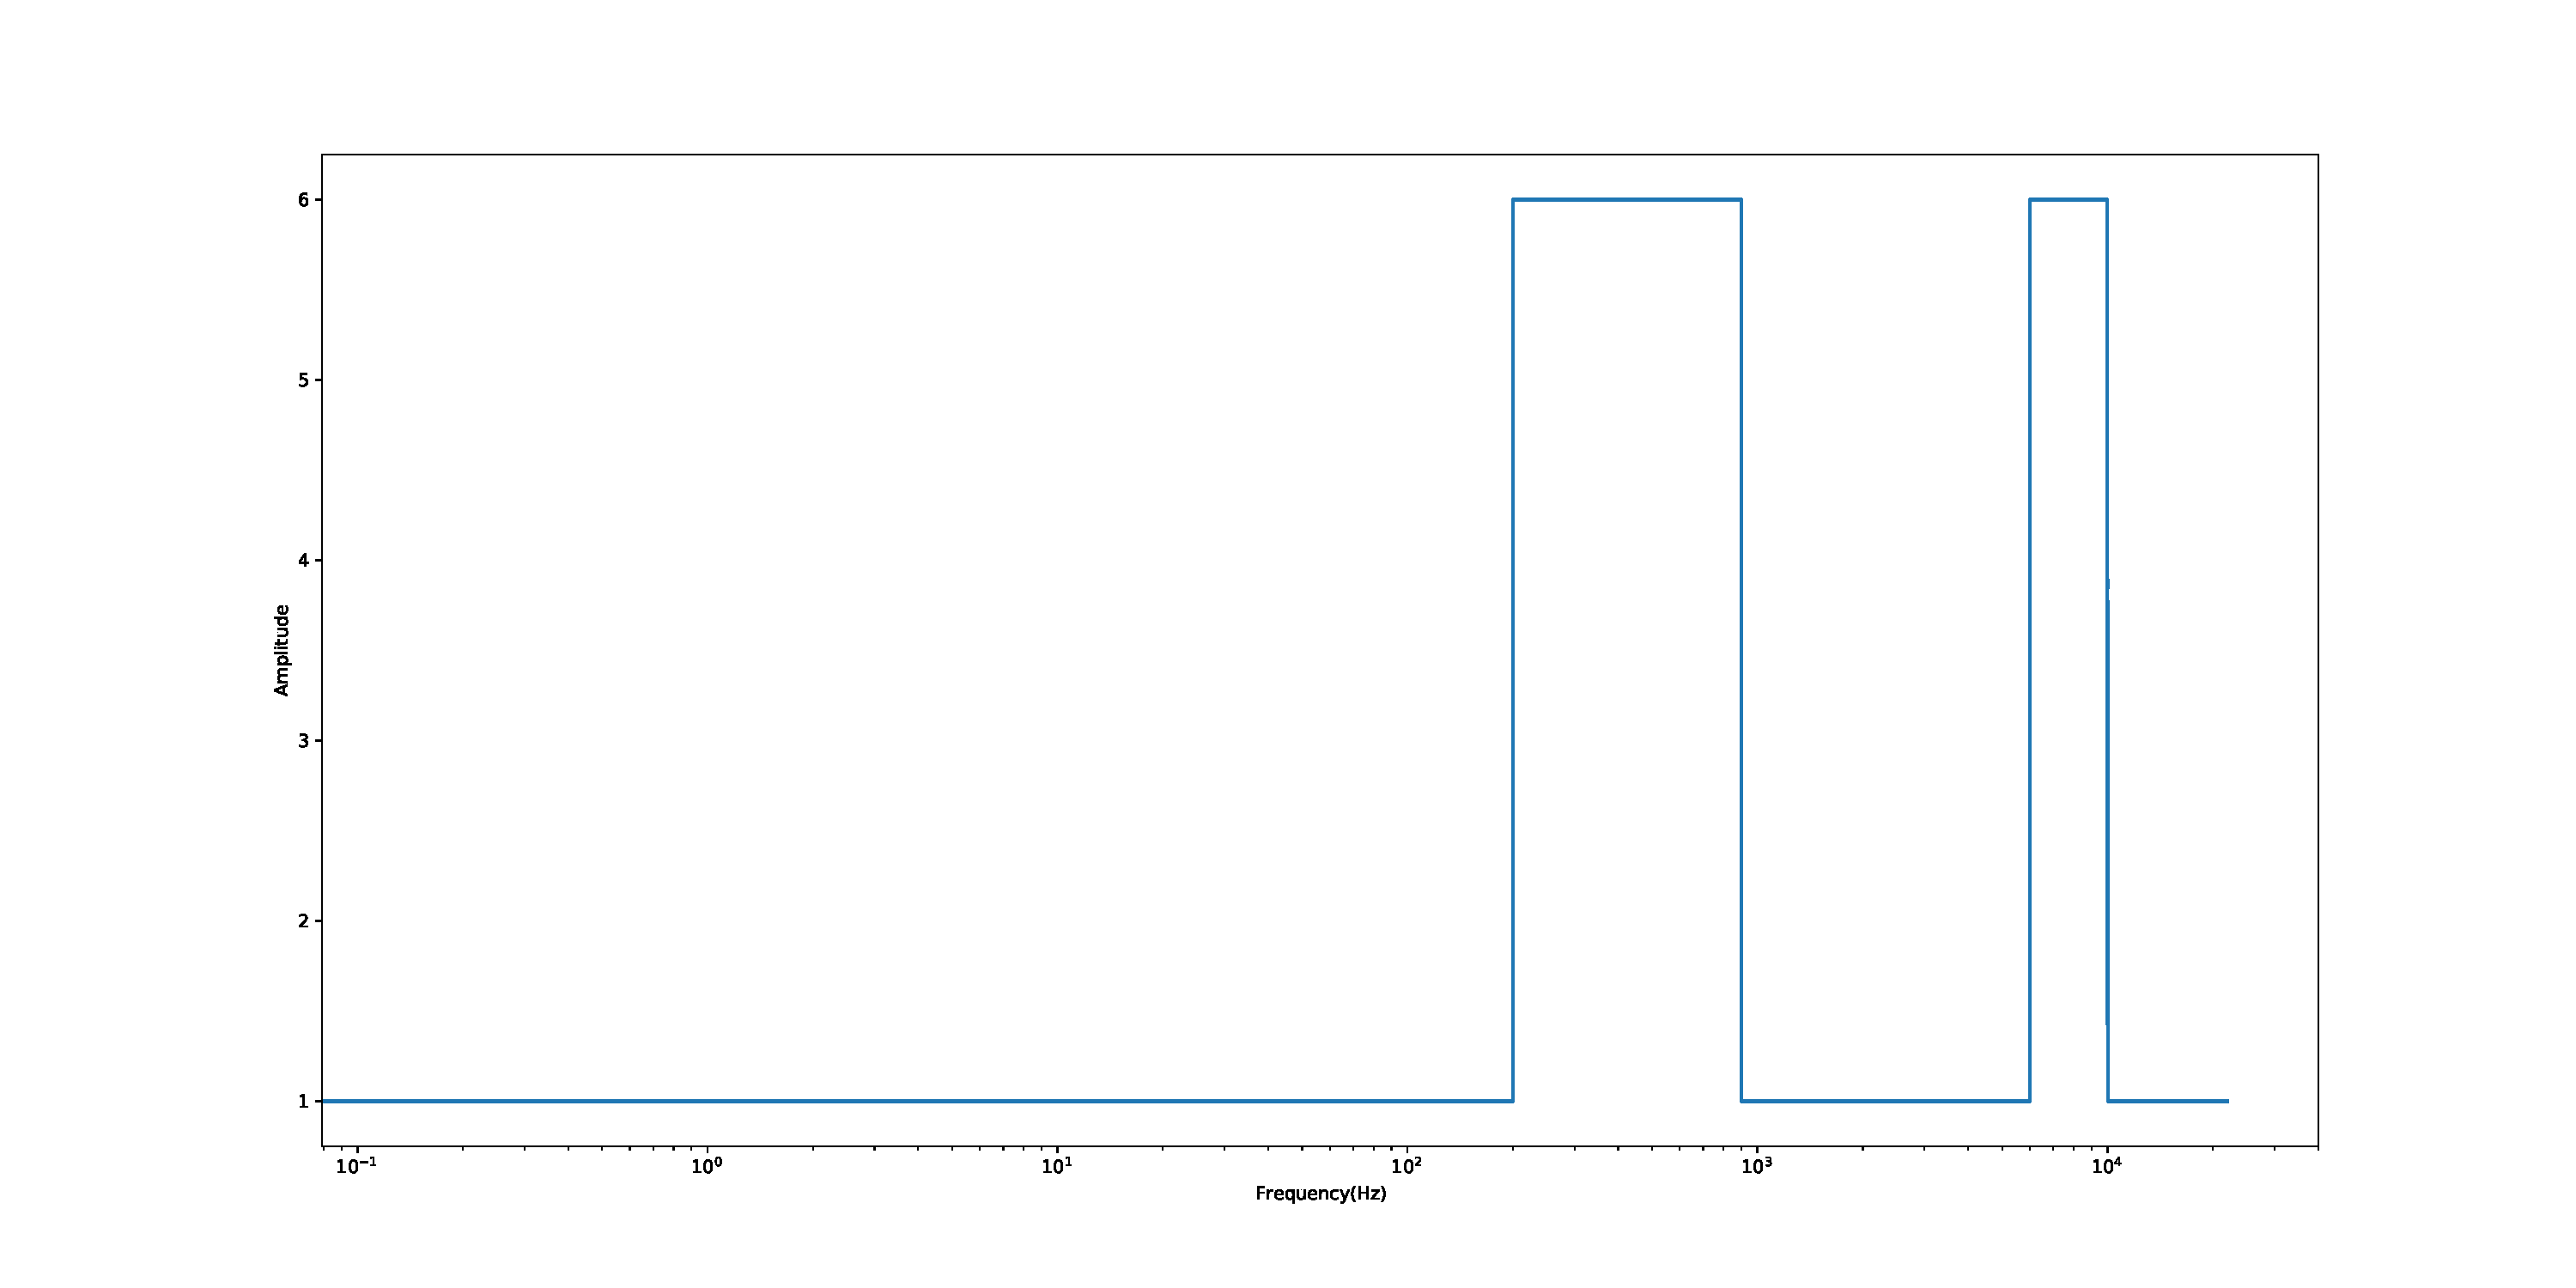
\includegraphics[width=12cm]{../Output/Figures/window.pdf} 
	\caption{window}   
	\label{fig_window}
\end{figure}
\begin{figure}[h]   
	\centering 
	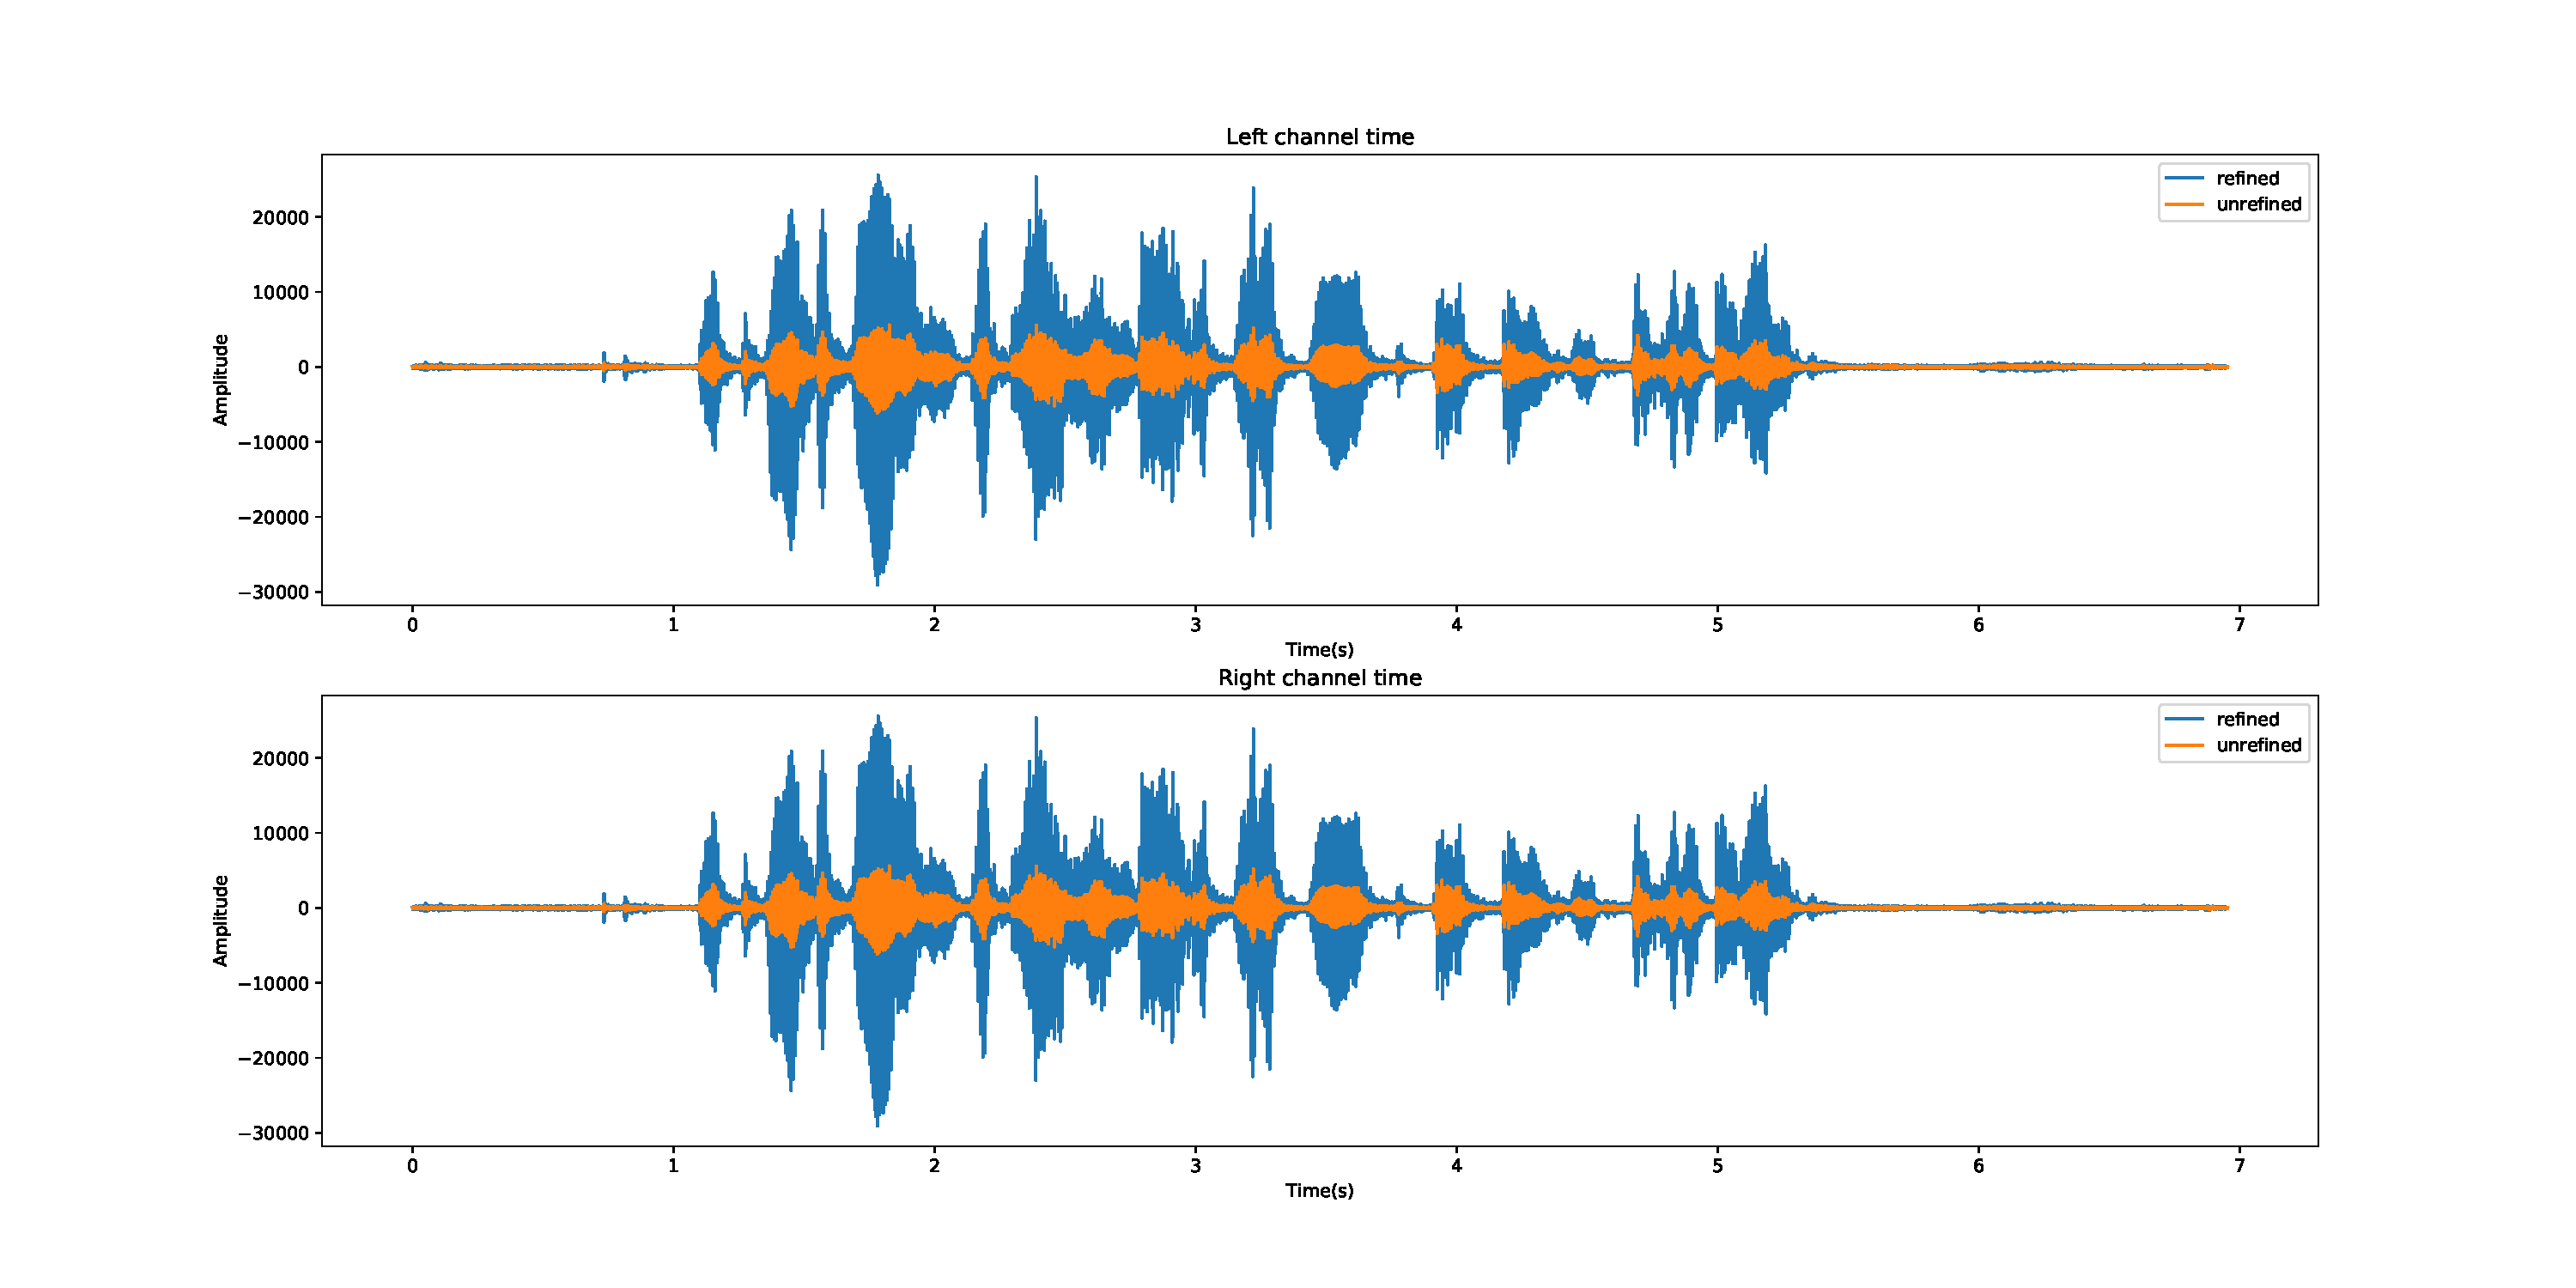
\includegraphics[width=12cm]{../Output/Figures/recordTR.pdf} 
	\caption{difference in time domain}   
	\label{fig_recordTR}
\end{figure}
\begin{figure}[h]   
	\centering 
	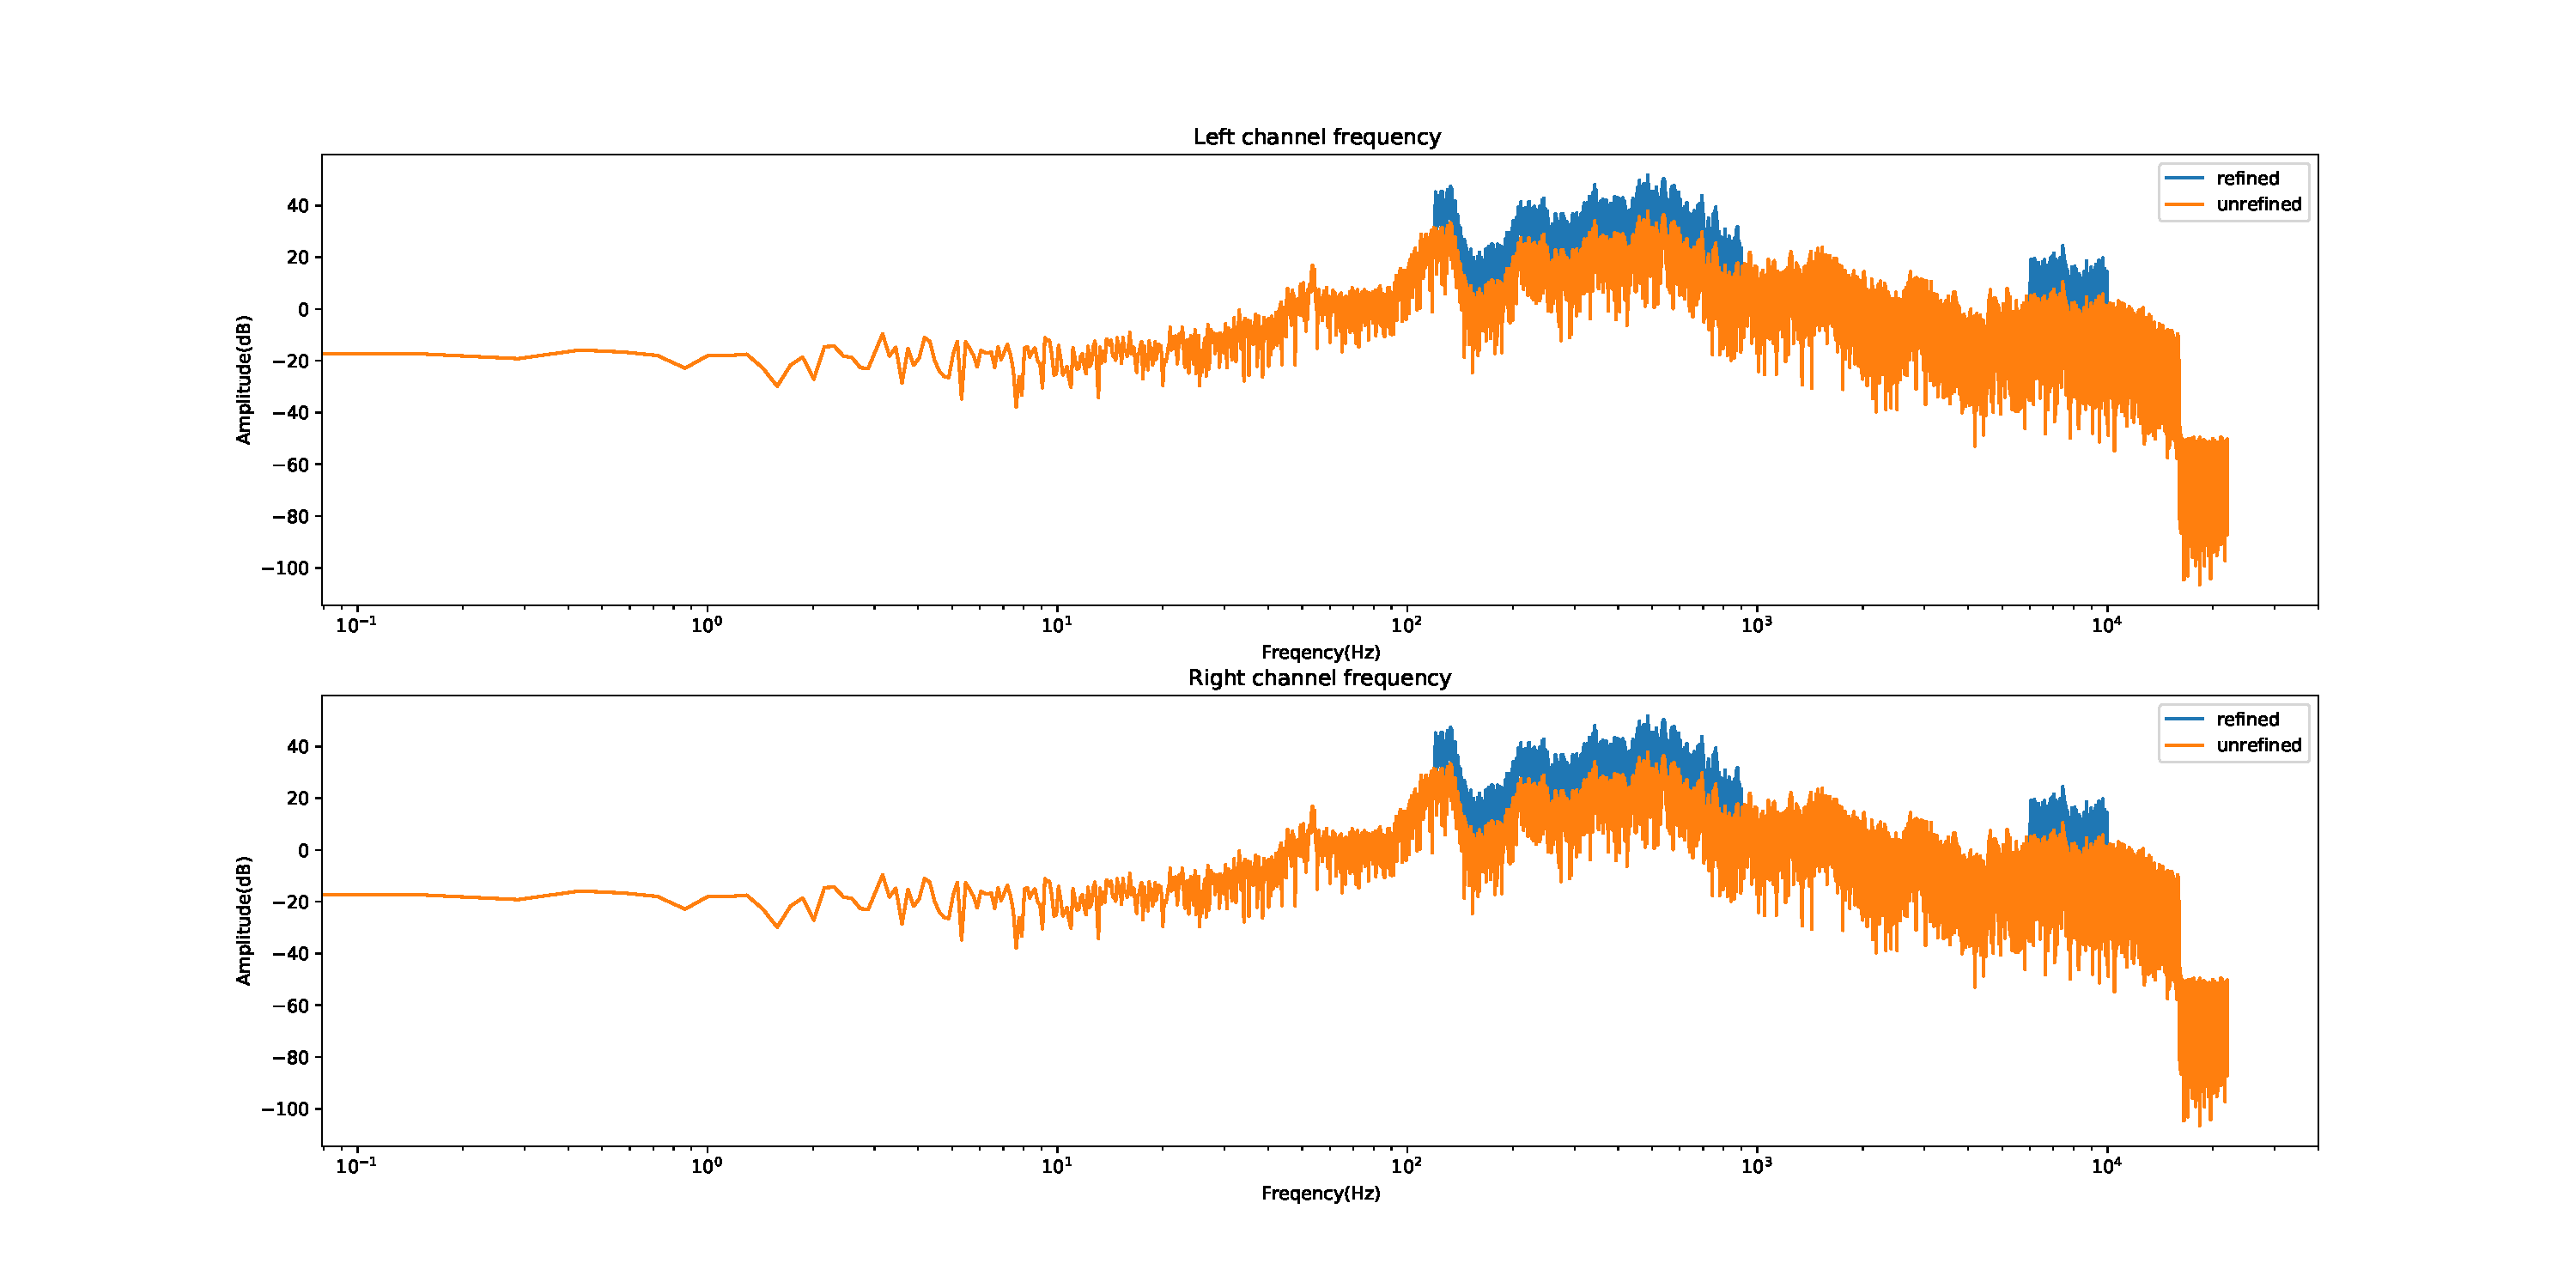
\includegraphics[width=12cm]{../Output/Figures/recordFR.pdf} 
	\caption{difference in frequency domain}   
	\label{fig_recordFR}
\end{figure}

\clearpage
\section{Task5}
\subsection{5.a}
The DTMF telephone keypad is laid out as a matrix of push buttons in which each row represents a low frequency component and each column represent a high frequency component of DTMF signal. So, in specific, we define the DTMF keypad as 3 data structures:
\begin{lstlisting}[language=Python]
dtmfHighFrequency = (1209, 1336, 1477, 1633)
dtmfLowFrequency = (697, 770, 852, 941)
dtmfLetter = [['1', '2', '3', 'A'],
								['4', '5', '6', 'B'],
								['7', '8', '9', 'C'],
								['*', '0', '#', 'D']]
\end{lstlisting}
Because frequencies of both higher and lower components are all greater than Nyquist frequency (500Hz), so we needed to convert them  into 0-500Hz using periodicity and symmetry property. \\
Secifically, we could convert the higher components by periodicity:
$$f_{convert}=f_{signal}-f_{samping}$$
And the lower component by symmetry:
$$f_{convert}=f_{sampling}-f_{signal}$$
In code:
\begin{lstlisting}[language=Python]
def aliasingFrequency(fs, sampleRate):
	"""convert the signal frequency into (0, N/2)"""
\end{lstlisting}
The frequency spectrum of a DTMF sinal has a distinct fearture. In the range of $[0,  f_{Nyquist}]$, it have 3 peaks, one is the DC component of the signal at 0Hz and the other two are belong to DTMF frequency (Figure\ref{fig_task5EampleF}).\\
\begin{figure}[h]   
	\centering 
	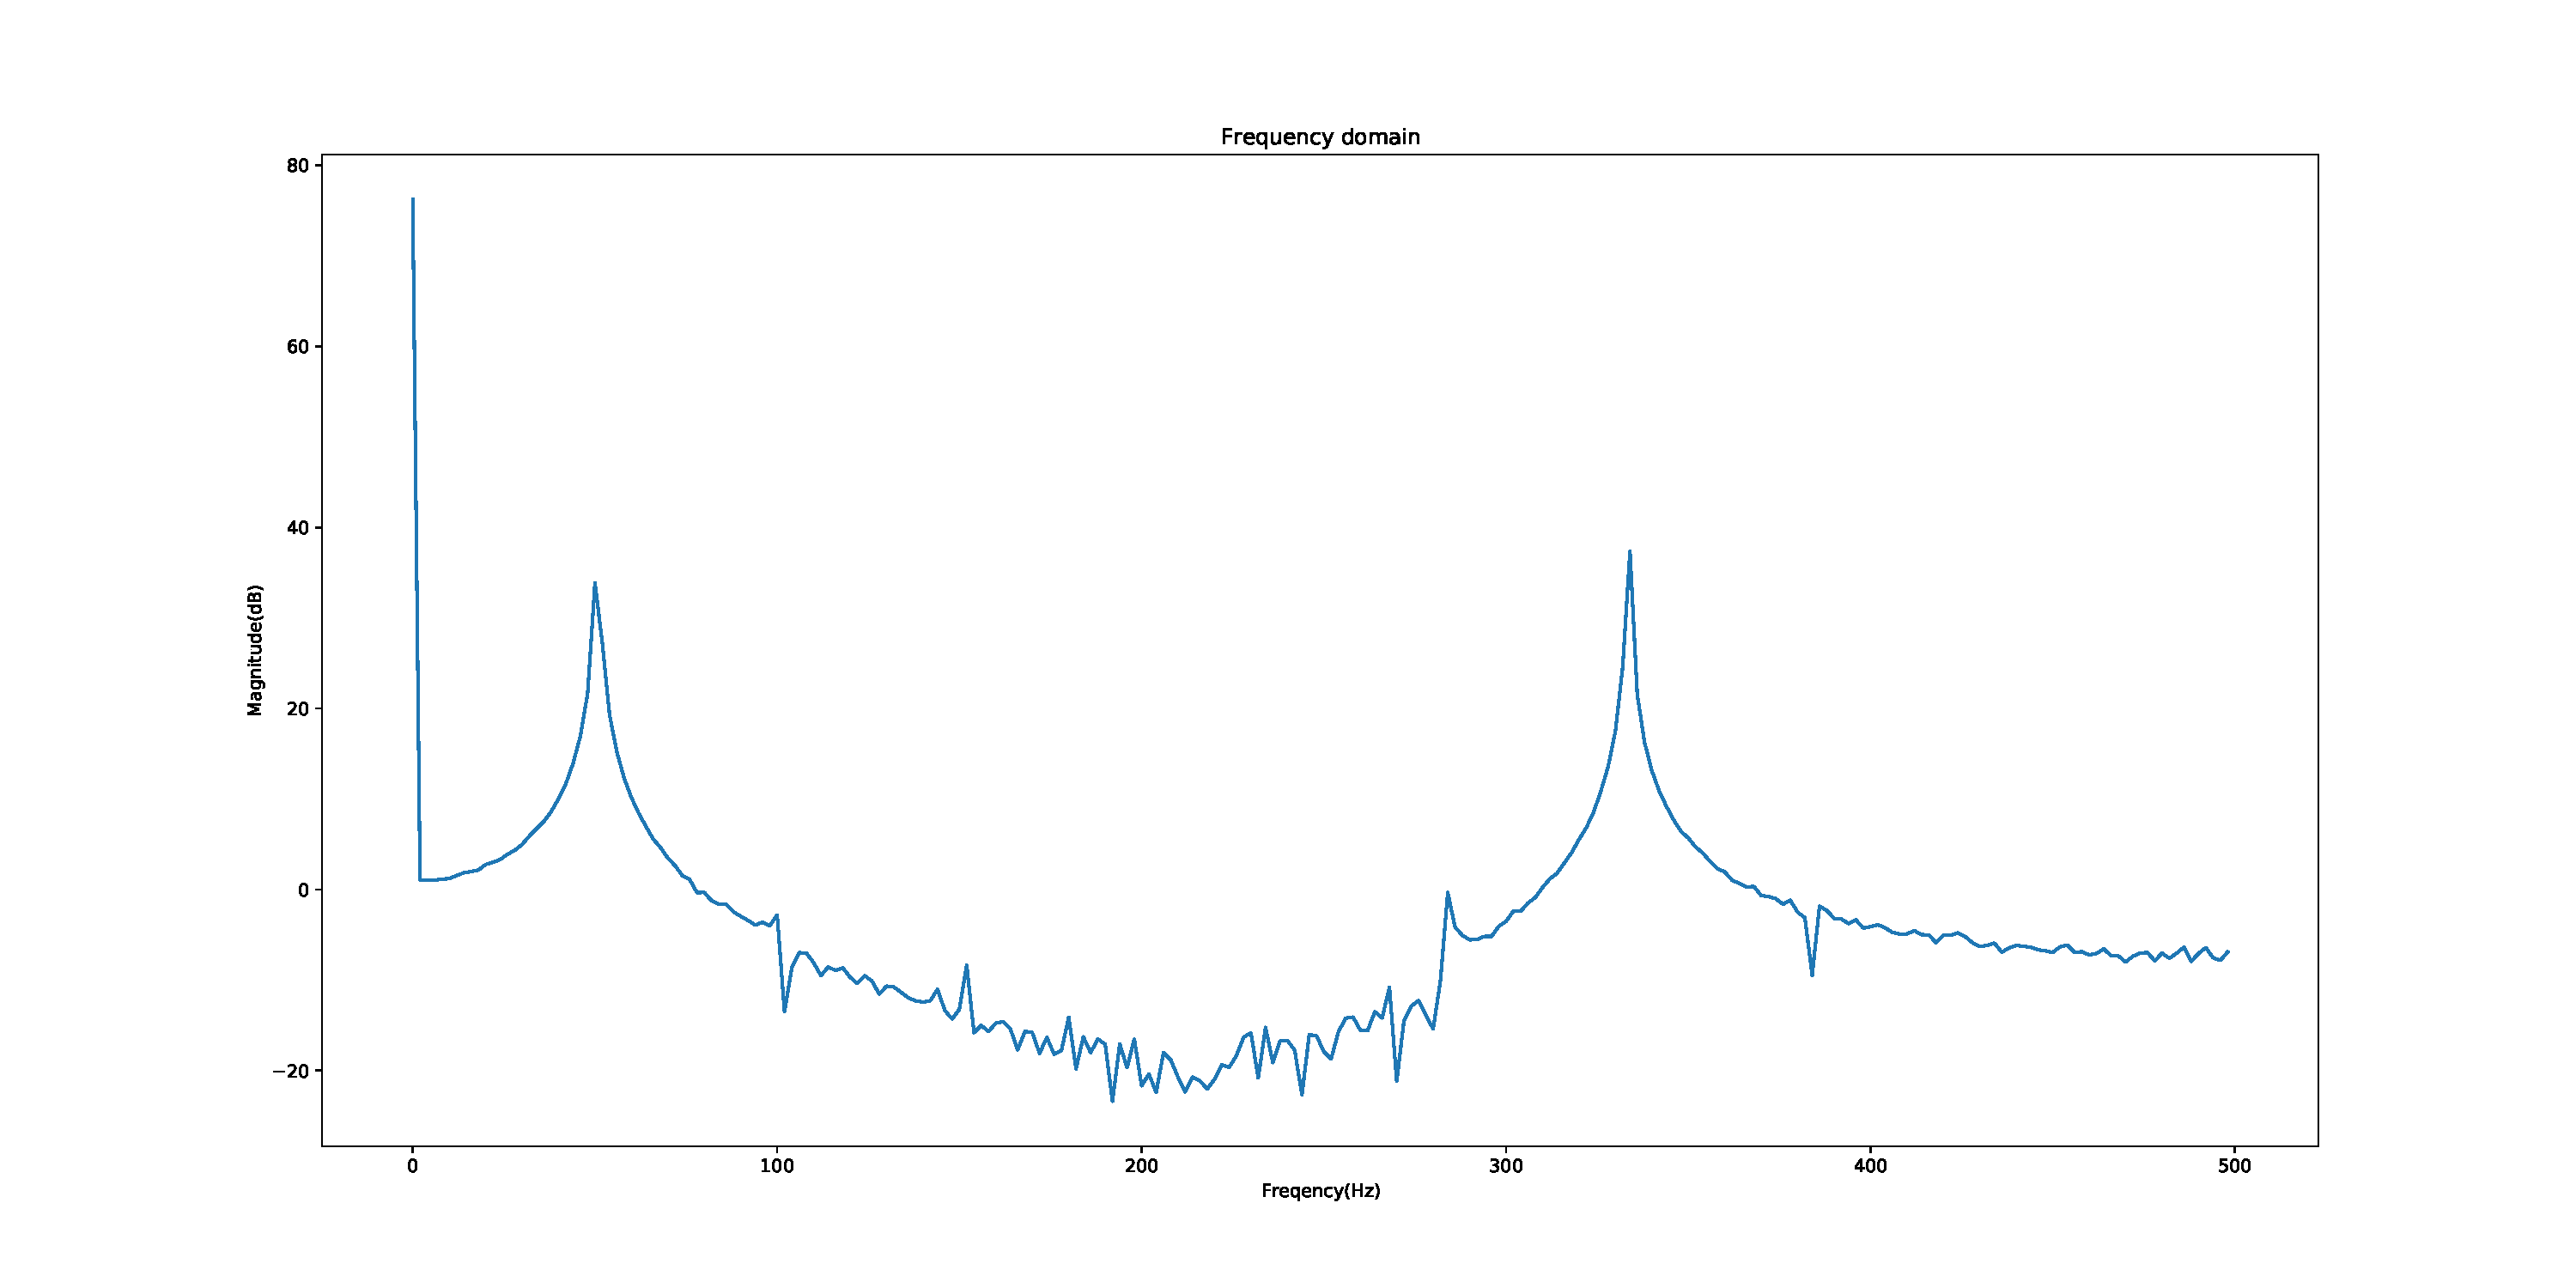
\includegraphics[width=12cm]{../Output/Figures/task5ExampleF.pdf} 
	\caption{frequency spectrum example of  single chunk}   
	\label{fig_task5EampleF}
\end{figure}
Thus, we need firstly find the 2 peaks:
\begin{lstlisting}[language=Python]
def peakFinding(data):
	"""find the max value of an array"""

def peakFindingDouble(data):
	"""find the first 2 greatest value of an array, except the 0 point"""
\end{lstlisting}
And figured out which DTMF component these peaks belonged:
\begin{lstlisting}[language=Python]
def findFrequencyBelong(f, dtmfMin, dtmfMax, sampleRate):
	"""
	Parameters
	---------
	f: 
	input frequency of the chunk signal
	dtmfMin: 
	acceptable lower bound 
	dtmfMax: 
	acceptable high bound
	sampleRate: 
	sampling frequency
	
	Returns
	------
	flag: 
	define which tone of the frequency belongs (high or low) 
	index: 
	return the index of dtmfFrequency array for easy finding of letter
	"""
\end{lstlisting}
After we found the index corresponding to the position in DTMF frequency list, we could easily find the number by:
\begin{lstlisting}[language=Python]
dtmfLetter[index1][index2]
\end{lstlisting}
Consequently, we could finish the function
\begin{lstlisting}[language=Python]
def detectOneDigitFromChunk(data, sampleRate):
"""
detect each chunk

Parameters
----------
data: ndarray
series of chunk data in time domain
sampleRate: float
the sampling frequency of signal

Returns
-------
letter: string
goal letter of this chunk 'N' means no letter found
"""
\end{lstlisting}
\subsection{5.b}
In the time domain, the signal \lstinline{"./Resources/TouchToneData/msc_matric_4"}could be plotted as Figure\ref{fig_DTMFtime}. We detected each chunk by rising edge. Specifically, we defined the length of each chunk as 300(300ms). A rising-edge chunk should be:
\begin{itemize}
\item the previous chunk should contains no DTMF number
\item this chunk should contains a legal DTMF number
\end{itemize}
In code:
\begin{lstlisting}[language=Python]
(preResult=='N') & (result != 'N')
\end{lstlisting}
Thus we could finish the function by while loop:
\begin{lstlisting}[language=Python]
def autoDetectNumbers(data, sampleRate):
	"""
	Parameters
	----------
	data : ndarray
	touch tone data
	sampleRate : int or float
	sampling frequency
	
	Returns
	-------
	seriesNumber : String
	the number detected
	"""
	while gap-1+K*gap < N:
	result = detectOneDigitFromChunk(data[K*gap: gap-1+K*gap], sampleRate)
	if((preResult=='N') & (result != 'N')):
	#print(K*gap*T,'s', "-", (gap-1+K*gap)*T,'s')
	seriesNumber = seriesNumber + result
	preResult = result
	K = K + 1
	return seriesNumber
\end{lstlisting}
Finally, the output is:
\begin{lstlisting}
start finding raising edge chunk
1.2 s - 1.499 s: 0
4.5 s - 4.799 s: 0
9.6 s - 9.899000000000001 s: 3
13.200000000000001 s - 13.499 s: 3
16.8 s - 17.099 s: 1
20.400000000000002 s - 20.699 s: 4
24.0 s - 24.299 s: 0
27.3 s - 27.599 s: 2
31.2 s - 31.499000000000002 s: 0
35.7 s - 35.999 s: 5
39.6 s - 39.899 s: 3
43.2 s - 43.499 s: 1
47.7 s - 47.999 s: 7
./Resources/TouchToneData/msc_matric_4.dat:
final result:  0033140205317
\end{lstlisting}

\begin{figure}[h]   
	\centering 
	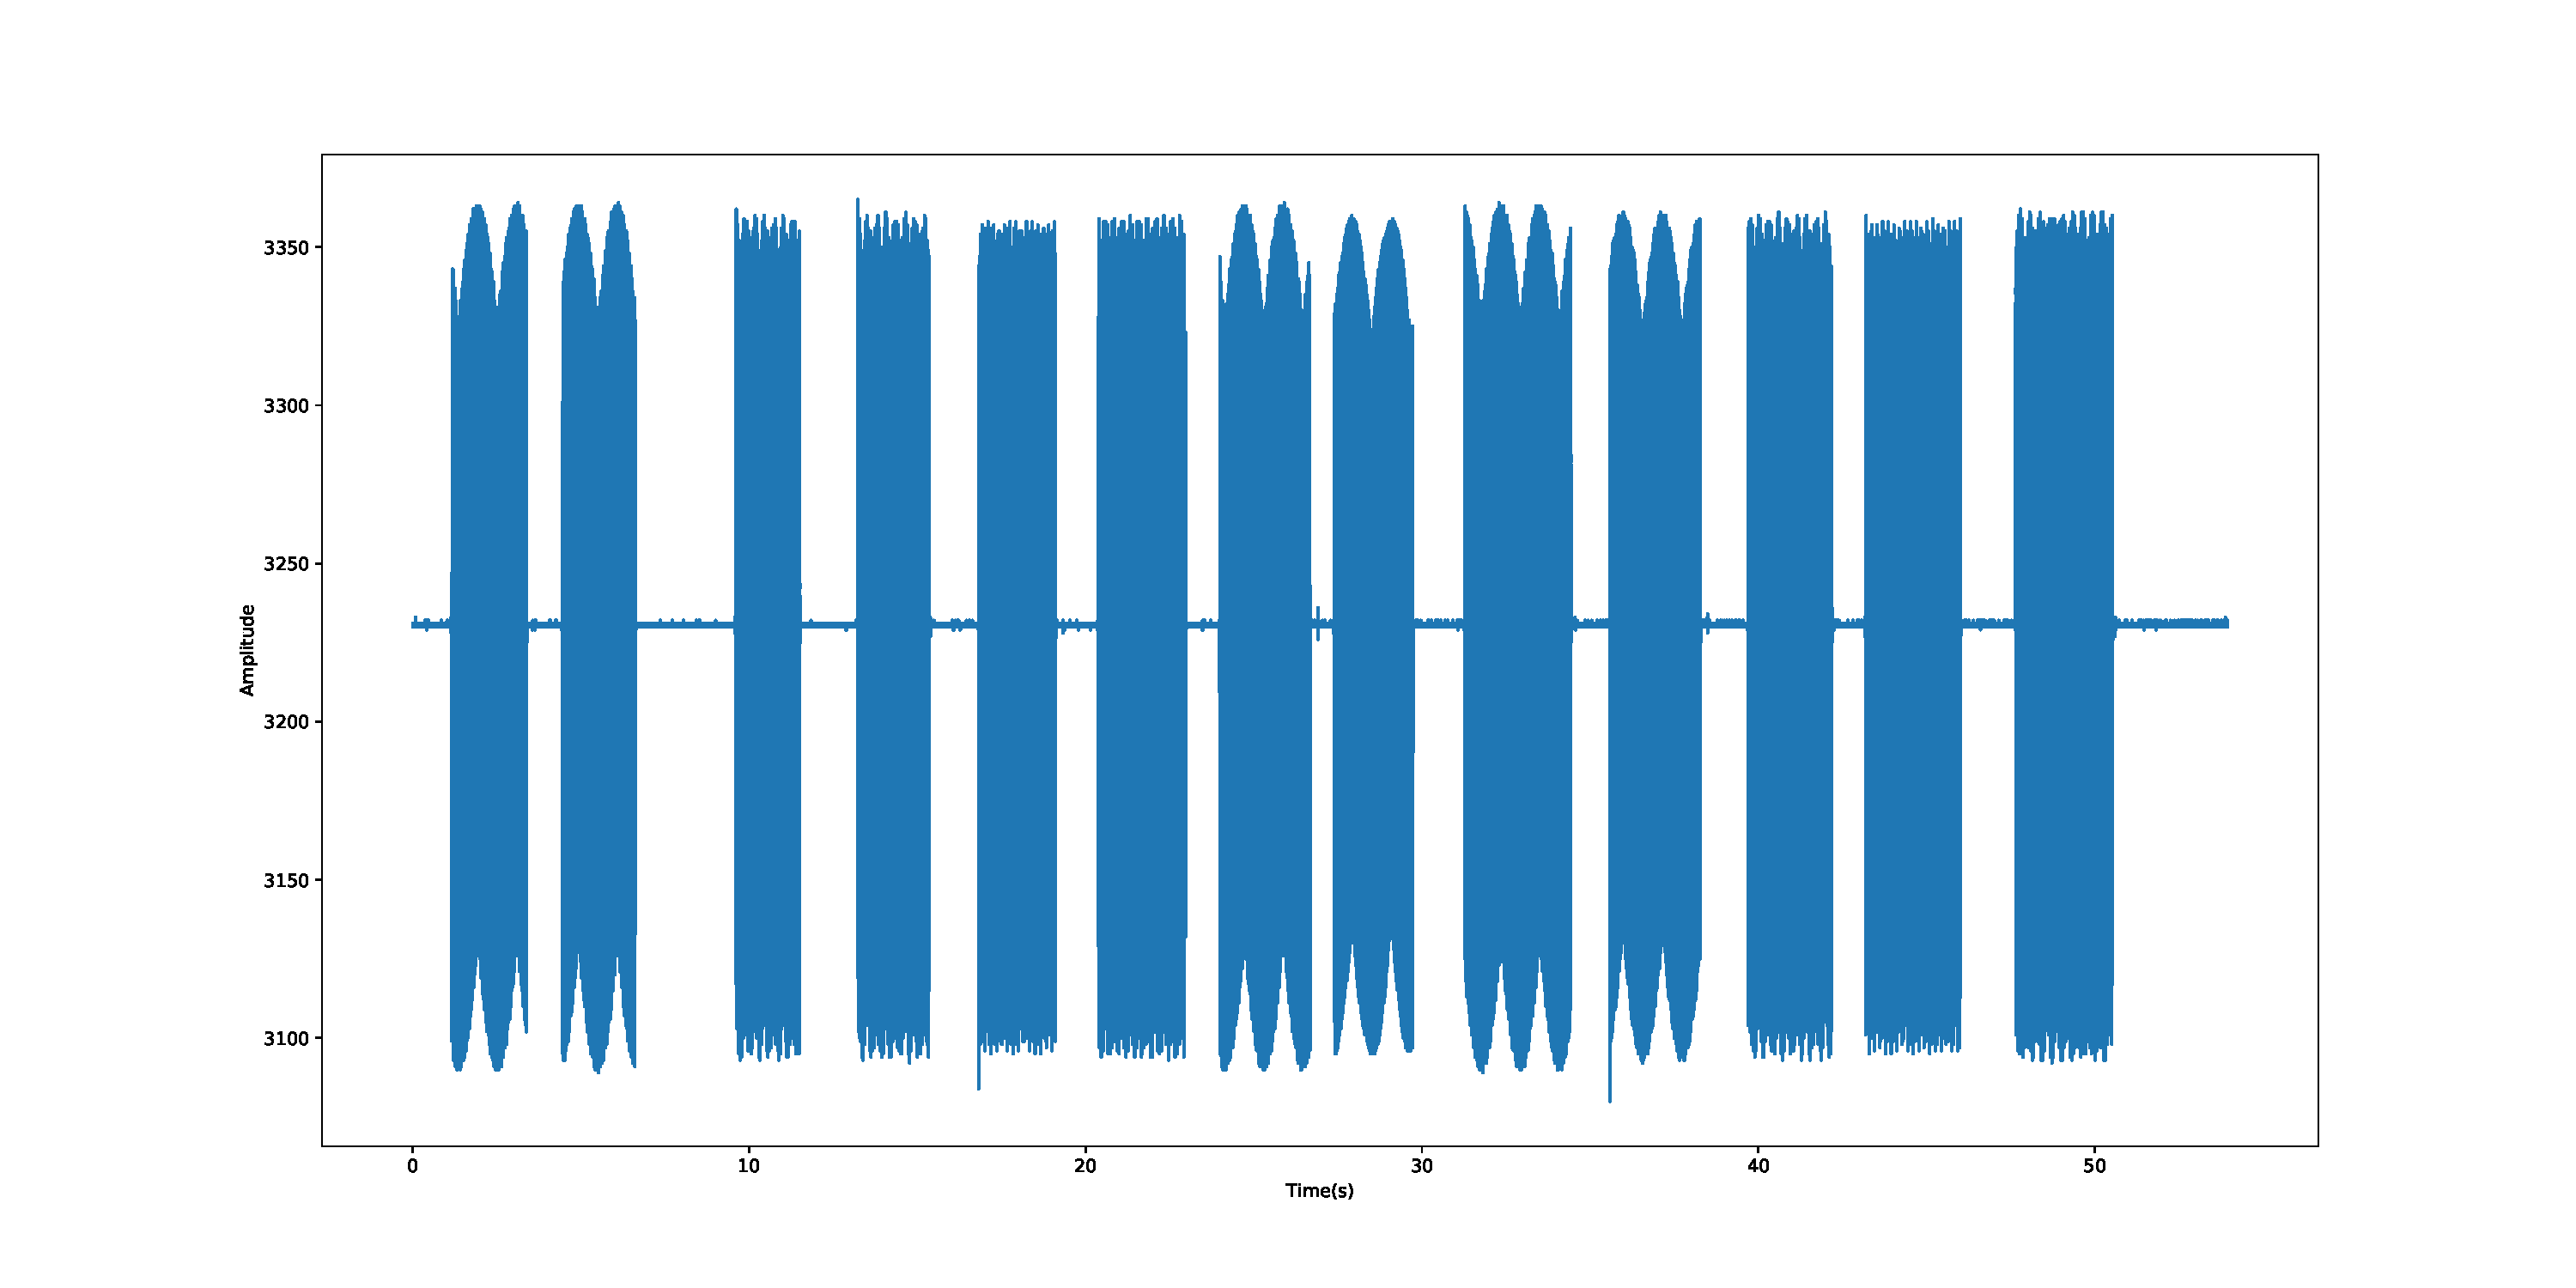
\includegraphics[width=12cm]{../Output/Figures/DTMFtime.pdf} 
	\caption{file msc matric 4}   
	\label{fig_DTMFtime}
\end{figure}

\clearpage
\section{Declaration of Originality and Submission Information}
I affirm that this submission is my own / the groups original work in accordance with the University of Glasgow Regulations and the School of Engineering Requirements.

\begin{itemize}
	\item Student Number: 2533494w\space Student Name: Jingyan Wang
	\item Student Number: 2595993w\space Student Name: Qianqian Wang
\end{itemize}

\clearpage
\section{Appendix}

\subsection{voiceEnhancer.py}
\lstinputlisting[language=Python]{../voiceEnhancer.py}
\subsection{touchToneDecoder.py}
\lstinputlisting[language=Python]{../touchToneDecoder.py}
\end{document}

